\documentclass[10 pt]{article}
\usepackage{tikz}
\usetikzlibrary{arrows}
\usepackage[margin=0.5 in]{geometry}
\usepackage[utf8]{inputenc}
\usepackage{tabu}
\usepackage{color}
\usepackage{mathtools}
\usepackage{amsfonts}
\usepackage{xcolor}
\usepackage{listings}
\usepackage{enumitem}
\usepackage{multicol}
\setlength{\columnsep}{1cm} 
\newtheorem{theorem}{Teorema}
\usepackage{mathrsfs}
\title{\textbf {Estructuras de Datos y Algoritmos 1 - ST0245\\Primer Parcial 002 - Martes}}
\author{Nombre ..............................\\
		Departamento de Informática y Sistemas\\
		Universidad EAFIT\\}
\date{Marzo 23 de 2021}
\begin{document}
% \lstdefinestyle{customc}{
% 	language=Java, 
% 	numbers=left, 
% 	showspaces=false,
%     showstringspaces=false, 
%     tabsize=2, 
%     breaklines=true,
%     xleftmargin=5.0ex,
% }
%\lstset{escapechar=@,style=customc, numbers=left, stepnumber = 1} 

\lstset{language=Java,frame=none, breaklines=true, numbers = left, stepnumber = 1, xleftmargin=5.0ex, showstringspaces=false, showspaces=false }
\lstset{language=Python,frame=none, breaklines=true, numbers = left, stepnumber = 1, xleftmargin=5.0ex, showstringspaces=false,showspaces=false }
\maketitle

\section{Mujeres en Ingeniería (2\% extra)}
 (2 \%) Varios estudios argumentan que muchas mujeres deciden NO estudiar ingeniería porque creen en los estereotipos sobre el tipo de personas que trabajan en el campo, y no se ven a sí mismas encajando en esos estereotipos. De esta manera, incorrectas percepciones pueden dar forma a las trayectorias profesionales. Una forma de desmentir dichos estereotipos es reconociendo mujeres exitosas en ingeniería de sistemas y matemática --tanto a nivel nacional como mundial. Para lograr esto, relaciona las siguientes mujeres con su contribución:


 \hspace{1cm}

% ANTERIORES
% 1. Marrisa Meyer &  a. Primera de Eafit en pasar a Google\\
% 2. María C. Choucair &  b. Primera gerente general de Yahoo \\
% 3. Ana Echavarría &  c. Primera de Eafit en pasar a Facebook \\
% 4. Kathie Bouman &  d. Código para el Apolo 11\\
% 5. Margaret Hamilton  & e. Primera foto de un agujero negro\\
% 6. Luisa M. Vásquez  &  f. Dueña de la empresa de \emph{testing} \\
% & más grande de Colombia


\begin{tabular}{l l}
1. Ada Lovelace &  a. Creadora de los procesadores ARM \\
2. Rózsa Péter &  b. Youtuber de algoritmos más vista\\
3. Gayle McDowell &  c. Primera en ganar un premio Turing\\
4. Dorothy Vaughan &  d. Primera persona en programar\\
5. Sophie Wilson &  e. Teoría de las funciones recursivas \\
6. Barbara Liskov &  f. Primera jefa de un equipo de computación en NASA \\
\\
 \end{tabular}
 



%Respuesta: 1 d, 2 e, 3 b, 4 f,  5 a, 6 c
1..., 2..., 3..., 4..., 5..., 6...



\newpage

\section{Recursión 30\%}
En la vida real, los algoritmos que trabajan sobre subsecuencias tienen una doble aplicación. Primero, se usan para analizar ADNs
en bioinformática; por ejemplo, para establecer la presencia de un desorden genético hereditario. Segundo, se utilizan para analizar
información de páginas web o redes sociales, como es el caso de Google, Facebook, Microsoft y Amazon. 
Te entregan dos cadenas de texto: $s$ y $t$. Encuentra el tamaño de la cadena más grande que es subsecuencia tanto de $s$ como $t$.
En una subsecuencia se respeta el orden de aparición de los caracteres, pero estos no aparecen --necesariamente-- de forma contigua. 
  Como un ejemplo, para las cadenas ``aa'' y ``xayaz'', la respuesta es $2$ porque la subsecuencia más larga es ``aa''.


 \hspace{1cm}


\textbf{Si trabajas en Java}, considera el siguiente código:

  \begin{lstlisting}[language=Java]
  int solve(String s, String t){
    return solve(s, t, s.length(), t.length()); 
  }
  int solve(String s, String t, int i, int j){
    if(i == 0 || j == 0) 
      return 0;
    if(s.charAt(i - 1) == t.charAt(j - 1))
      return .........................;
    //else
    return .........................;
  }
  \end{lstlisting}
  

  \textbf{Si trabajas en Python}, considera el siguiente código:

  \begin{lstlisting}[language=Python]
  def mainSolve( s,  t):
    return solve(s, t, len(s), len(t)) 
  
  def solve(s, t, i, j):
    if i == 0 or j == 0: 
       return 0;
    if s[i - 1] == t[j - 1]:
      return .........................
    else:
      return .........................
  }
  \end{lstlisting}

  \begin{enumerate}[label=(\Alph*)]
    % Solución: 1 + solve(s, t, i - 1, j - 1)
    \item (10\%) Completa la línea 8 \\ \\
    \line(1, 0){230}
    % Solución
    % Java: Math.max(solve(s, t, i, j - 1), solve(s, t, i - 1, j))
    % Python: max(solve(s, t, i, j - 1), solve(s, t, i - 1, j))
    \item (10\%) Completa la línea 10 \\ \\
    \line(1, 0){230}
    % Solución: T(n) = T(n-1) + T(n-1), que es O(2^n)
    \item (10\%) ¿Cuál es la complejidad asintótica para el peor de los casos? \\ \\
    T(n) = \line(1, 0){210} , donde $n$ es la suma de la longitud de $s$ y $t$.
  \end{enumerate}

\newpage




\section{Notación O 20\%}
En la vida real,  hacemos filas de espera (\textit{Waiting lines}) para entrar a un parqueadero, para ser atendido en un banco o para comprar un producto en un supermercado.
 Implementar filas de espera, en un programa informático, es importante para simular, por ejemplo, el impacto que tendría
 --sobre los tiempos de espera-- el contratar un nuevo cajero. Por eso, estas implementaciones son de suma importancia para empresas como Bancolombia. 
La siguiente clase implementa una fila de espera para un máximo de $n$ elementos. Tan sólo hace falta calcular la complejidad asintótica, para el peor de los
casos, de las operaciones entrar a la fila de esperar (\textit{enqueue}) y salir de la fila de espera (\textit{dequeue}). 

\hspace{1 cm}

\textbf{Si trabajas en Java}, considera el siguiente código:

\begin{lstlisting}[language = Java]
class WaitingLine {
  int e[];
  int index;
  boolean started;

  WaitingLine(int n) {
    e = new int[n];
    index = 0;
    started = false;
  }

  public boolean isEmpty() {
    return (index == 0 && !started) | index <= 0;
  }

  void enqueue(int x){
    if (index == e.length) {
      throw new RuntimeException("Full");
    }
    started = true;
    e[index] = x;
    index++;
  }

  int dequeue(){
    if (isEmpty())
      throw new RuntimeException("Empty");
    int x = e[0];
    for (int i = 0; i < index - 1; i++) {
      e[i] = e[i + 1];
    }
    index--;
    return x;
  }
}
\end{lstlisting}

\begin{enumerate}[label=(\Alph*)]
  % O(1)
  \item (10\%) Calcula la complejidad asintótica, para el peor de los casos, de 
   \texttt{enqueue(x)} \\ \\
   O(\line(1, 0){230})\\

  % O(n)
  \item (10\%) Calcula la complejidad asintótica, para el peor de los casos, de 
   \texttt{dequeue(x)} \\ \\
   O(\line(1, 0){230})\\


\end{enumerate}

\newpage

\textbf{Si trabajas en Python}, considera el siguiente código:

\begin{lstlisting}[language = Python]
import numpy as np
class WaitingLine:

  def __init__(self, n):
    self.e = np.zeros(n)
    self.index = 0;
    self.started = False;

  def isEmpty(self): 
    return (self.index == 0 and not self.started) or self.index <= 0

  def enqueue(self,x):
    if self.index == self.e.size:
      raise Exception("Full")
    self.started = True
    self.e[self.index] = x
    self.index = self.index + 1

  def dequeue(self):
    if self.isEmpty():
      raise Exception("Empty")
    x = self.e[0]
    for i in range (0, self.index - 1):
      self.e[i] = self.e[i + 1]
    self.index = self.index - 1
    return x
\end{lstlisting}




\begin{enumerate}[label=(\Alph*)]

  \item (10\%) Calcula la complejidad asintótica, para el peor de los casos, de 
   \texttt{enqueue(x)} \\ \\
   O(\line(1, 0){230})\\

  \item (10\%) Calcula la complejidad asintótica, para el peor de los casos, de 
   \texttt{dequeue(x)} \\ \\
   O(\line(1, 0){230})\\


\end{enumerate}

\newpage

\section{Listas enlazadas 20\%}

La \textit{Notación polaca inversa} es una notación matemática en la cual los operadores siguen sus operandos. En la vida real, la notación polaca inversa fue ampliamente utilizada, en los años 70s y 80s, por las calculadoras científicas 
Hewlett-Packaar. Por ejemplo, la expresión en notación polaca $5\;31\;4 + \times$, equivale a la expresión $(31 + 4) \times 5$. Dado  un arreglo de operadores y operandos (\textit{tokens}) que representan una expresión en notación polaca, considerando sólo  los operadores ``(+, *, -, /)'', determina el resultado de la expresión. Utilizando una lista enlazada, es posible operar una expresión en notación, así:

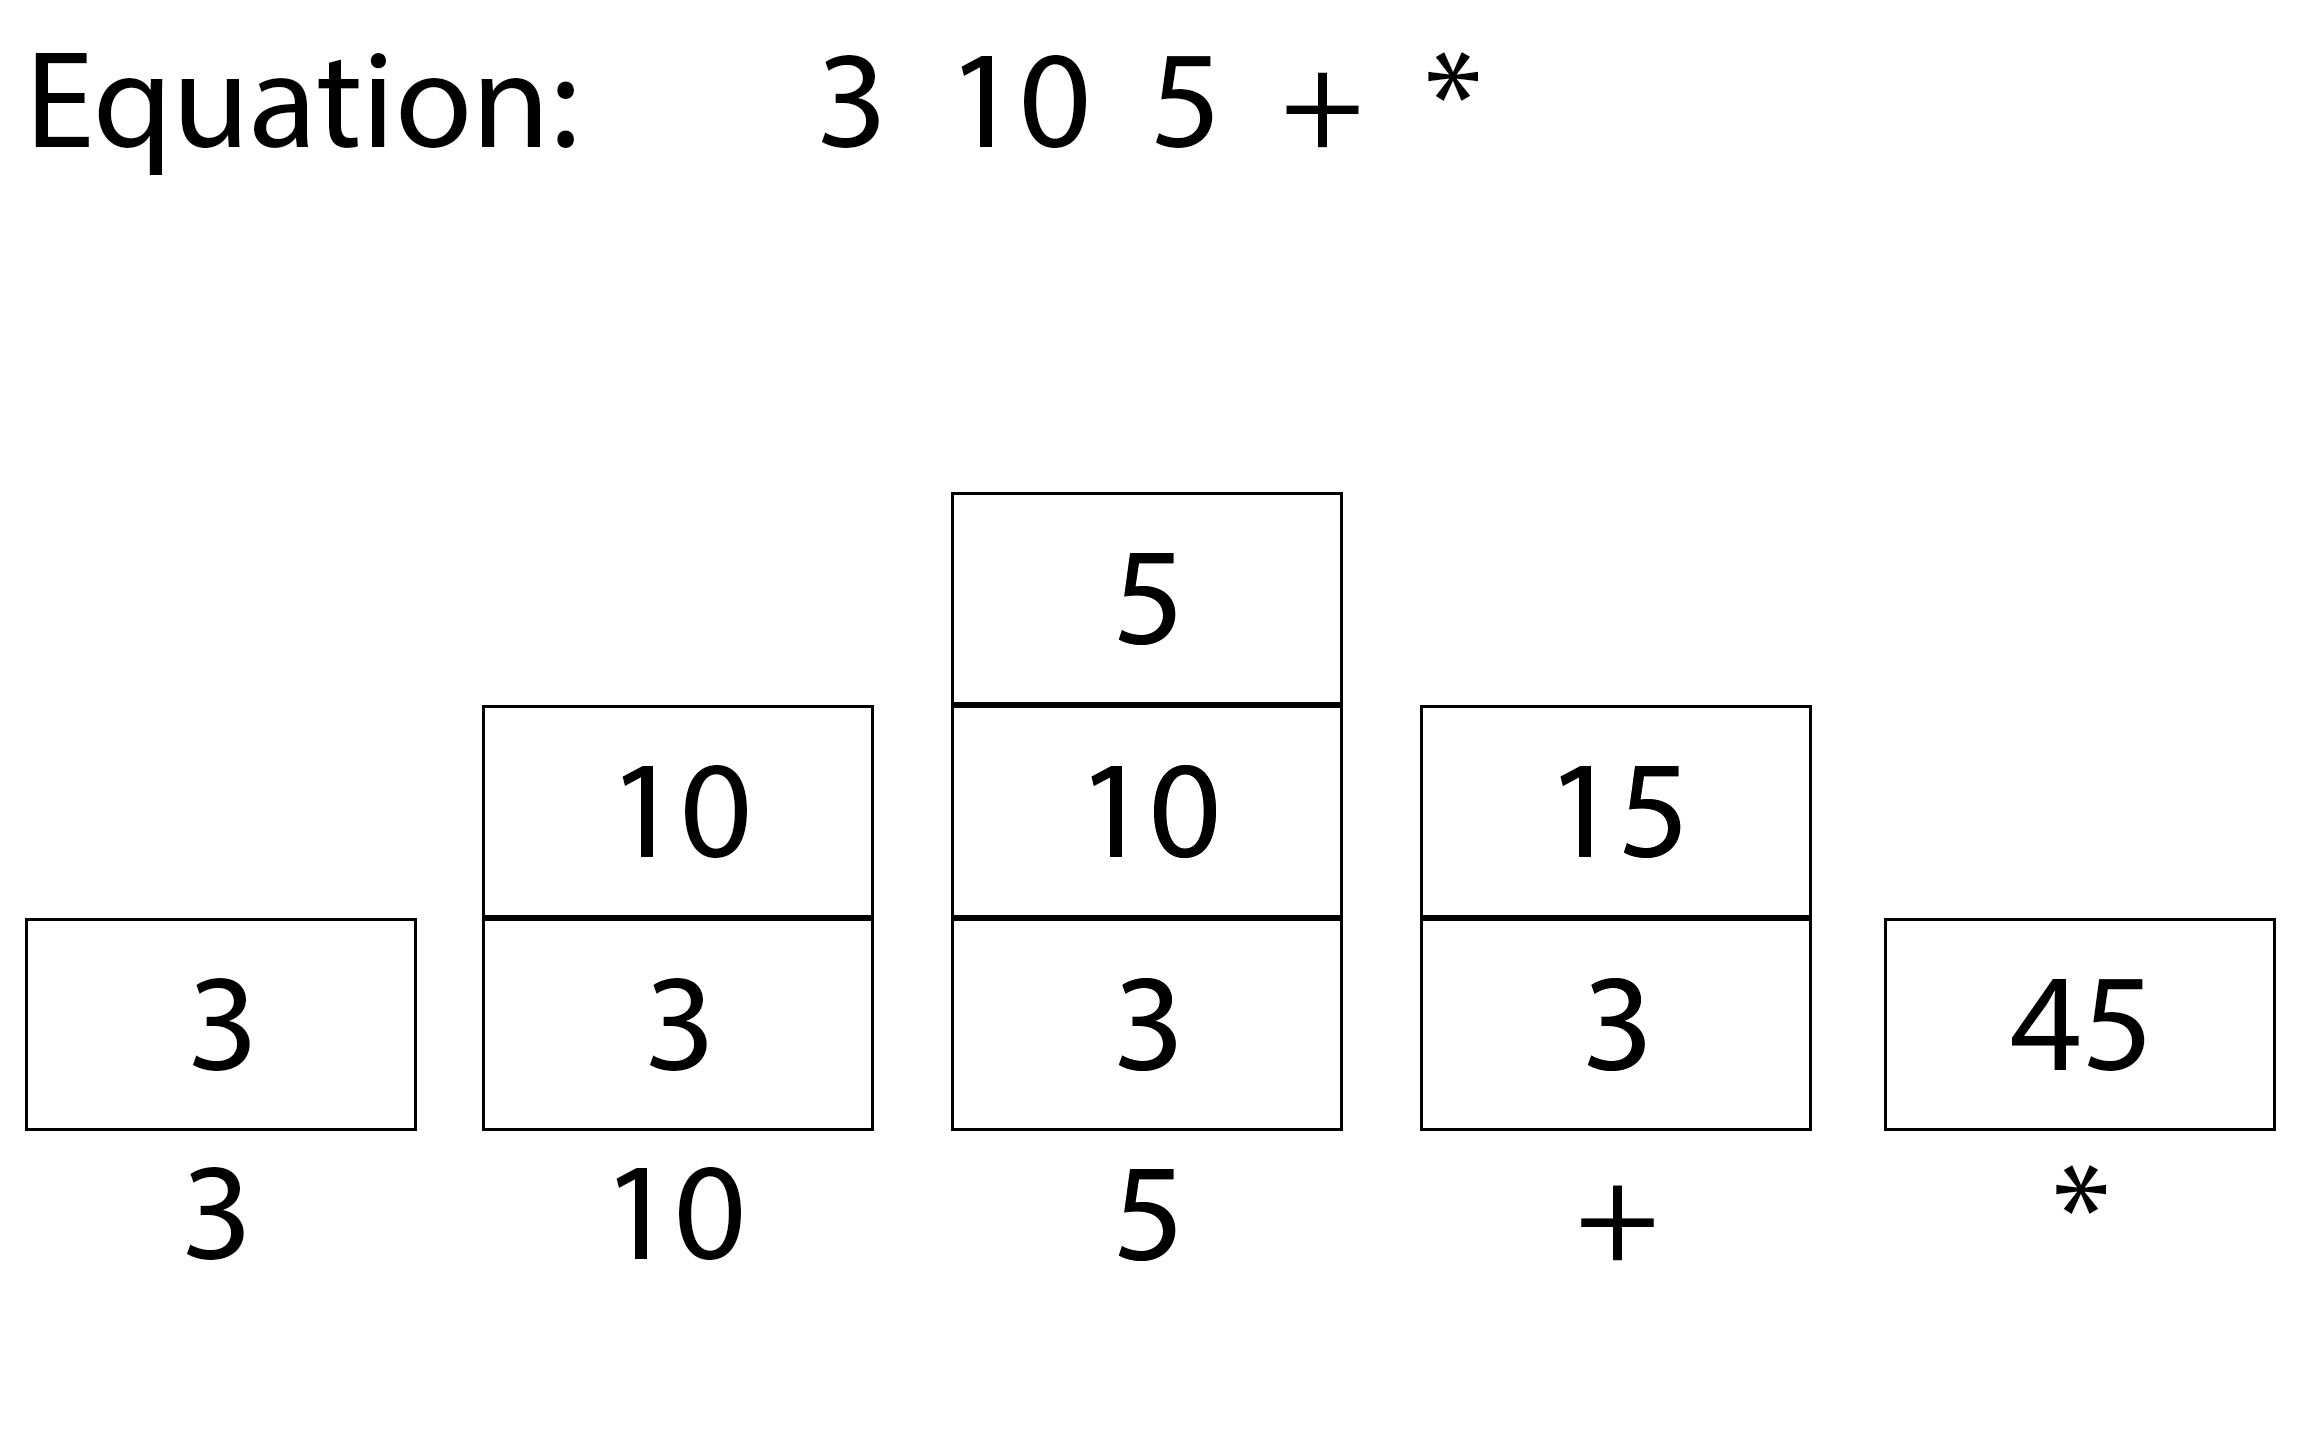
\includegraphics[scale=0.07]{ReversePolishNotationStackExample.jpg}


Ya hemos adelantado algo de trabajo, pero falta completar algunas líneas, por favor.

\hspace{1 cm}

\textbf{Si trabajas en Java}, considera el siguiente código:

\begin{lstlisting}[language = Java]
int solve(String[] tokens){
  String operators = "+-*/";
  LinkedList<String> aList = new LinkedList<String>();
  for(String t : tokens){
    if(!operators.contains(t)){
      ..............;
    }else{
      int a = ..................;
      aList.remove(0);
      int b = ..................;
      aList.remove(0);
      int index = operators.indexOf(t);
      if(index == 0) 
       aList.add(0,String.valueOf(a+b));
      else if(index == 1)
       aList.add(0,String.valueOf(b-a));
      else if(index == 2)
       aList.add(0,String.valueOf(a*b));
      else // index == 3
       aList.add(0,String.valueOf(b/a));
    }
  }
  String last = aList.remove(0);
  return ...............;
}
\end{lstlisting}
\begin{enumerate}[label=(\Alph*)]
 
  % Solución Java: aList.add(0,t)
  \item (10\%) Completa la línea 6\\
  \line(1, 0){230}\\
  % Solución Java: Integer.valueOf(aList.get(0)),Integer.valueOf(aList.get(0))
  \item (10\%) Completa las líneas 8 y 10\\
  \line(1, 0){230} \\
  \line(1, 0){230}\\
  % Solución Java: Integer.valueOf(last)
  Y completa la línea 24\\
  \line(1, 0){230}
\end{enumerate}

En Java, el método \texttt{String.valueOf(a)} convierte el entero $a$ en una cadena de caracteres y el método \texttt{Integer.valueOf(b)} convierte la cadena $b$ en un entero.

\newpage

\textbf{Si trabajas en Python}, considera el siguiente código:

\begin{lstlisting}[language = Python]
def solve(tokens):
  operators = "+-*/"
  aList = []
  for t in tokens:
    if not t in operators:
      ..................
    else:
      a = .........
      aList = aList[1:]
      b = ..........
      aList = aList[1:]
      index = operators.index(t)
      if index == 0:
       aList = [str(a+b)] + aList 
      elif index == 1:
       aList = [str(a-b)] + aList 
      elif index == 2:
       aList = [str(a*b)] + aList 
      else:
       aList = [str(b/a)] + aList 
  last = aList[0]
  return ...............
\end{lstlisting}

\begin{enumerate}[label=(\Alph*)]
 
  % Solución: aList = [t] + aList
  \item (10\%) Completa la línea 6\\
  \line(1, 0){230}\\
  % Solución: int(aList[0])   y   int(aList[0])
  \item (10\%) Completa las líneas 8 y 10\\
  \line(1, 0){230} \\
  \line(1, 0){230}\\
  % Solución: int(last)
  Y completa la línea 22\\
  \line(1, 0){230}
\end{enumerate}

En Python, la función \texttt{str(a)} convierte el entero $a$ en una cadena de caracteres y la función \texttt{int(b)} convierte la cadena $b$ en un entero.

\newpage

\section{Vectores dinámicos 10\%}

Empresas como Microsoft se benefician muchísimo de los algoritmos basados en subarreglos, por ejemplo, para implementar el algoritmo de \textit{buscar} o \textit{reemplazar} en sus programas ofimáticos. Pensemos un problema con subarreglos. Dado un arreglo \texttt{arr} de \texttt{n} enteros, encuentra, por favor, el subarreglo contiguo con la máxima suma posible. Este problema, coincidencialmente, es muy común en entrevistas de Microsoft, Oracle y Amazon según el portal \textit{Geeks for Geeks}. Como un ejemplo, si tenemos el arreglo $arr = \{1,2,3,-2,5\}$, la respuesta es $9$ porque todo el arreglo es el subarreglo con la máxima suma. Como otro ejemplo, si tenemos el arreglo $arr = \{-1, -2, -3, -4 \}$, la respuesta es $-1$ porque el subarreglo
con máxima suma es $\{-1\}$. Hemos avanzado un poco, pero falta una línea. Complétala, por favor. Gracias.

\hspace{1cm}

\textbf{Si trabajas en Java}, considera el siguiente código:

\begin{lstlisting}[language = Java]
int maxSubArraySum(ArrayList<Integer> a)
{
        int size = a.size();
        int max_so_far = Integer.MIN_VALUE, max_ending_here = 0;
 
        for (int i = 0; i < size; i++)
        {
            max_ending_here = max_ending_here + a.get(i);
            if (.......................) 
                max_so_far = max_ending_here;
            if (max_ending_here < 0)
                max_ending_here = 0;
        }
        return max_so_far;
    }
}
\end{lstlisting}

En Java, \texttt{Integer.MIN\_VALUE} representa el entero más pequeño.

\hspace{1cm}

\textbf{Si trabajas en Python}, considera el siguiente código:

\begin{lstlisting}[language=Python]
import math
def maxSubArraySum(a,size):
      
    max_so_far = -1*math.inf - 1
    max_ending_here = 0
      
    for i in range(0, size):
        max_ending_here = max_ending_here + a[i]
        if (....................):
            max_so_far = max_ending_here
 
        if max_ending_here < 0:
            max_ending_here = 0  
    return max_so_far
  
\end{lstlisting}

En Python, \texttt{math.inf} representa el infinito ($\infty$) y \texttt{-1*math.inf} el menos infinito ($-\infty$).

  \begin{enumerate}[label=(\Alph*)]
    % Solución Java y Python: max_so_far < max_ending_here
    \item (10\%) Completa la línea 9\\ \\
    \line(1, 0){230}
    
  \end{enumerate}


\newpage

\section{Complejidad 20\%}
En empresas como Riot Games, Electronic Arts y Microsoft, para entrar a trabajar como desarrollador de videojuegos, es imperativo conocer sobre complejidad de algoritmos. Considera el siguiente algoritmo:

\hspace{1cm}

\textbf{Si trabajas en Java}, considera el siguiente código:

\begin{lstlisting}[language=Java]
void doSomething(int n){
  int sum = 0;
  for(int i = 1; i <= n; ++i){
    for(int j = i + 1; j <= n; j = j * 2){
      sum ++;
    }
  }
}
\end{lstlisting}

\textbf{Si trabajas en Python}, considera el siguiente código:

\begin{lstlisting}[language=Python]
def doSomething(n):
  sum = 0
  for i in range(1, n+1):
    j = i+1
    while j <= n:
      sum = sum + 1;
      j = j * 2
\end{lstlisting}

\begin{enumerate}[label=\alph*]
% Respuesta: O(n log n)
\item (10\%) Calcula la complejidad asintótica, para el peor de los casos, es decir, $O(T(n))$: O(......................)
% Respuesta: O(n)
\item (10\%) Calcula la complejidad asintótica, para el peor de los casos, si cambiamos \texttt{j = j * 2} por \texttt{j = j + 2}: O(......................)
\end{enumerate}

\newpage

\section{Complejidad (10\% EXTRA)} 



El desarrollo de juegos es de suma importancia para empresas como \textit{Riot Games} y \textit{Microsoft}. Consideremos el siguiente juego. 
Hay $n$ muros donde María Isabel va a empezar a saltar. María se encuentra en el muro $1$ y quiere llegar al muro $n$. Sí María se encuentra en el muro $i$, solo puede saltar a los muros $i + 1, i + 2, \cdots, i + k$. Al realizar el salto --desde el muro $i$ hasta el muro $j$--, ella gasta $\mid a_i - a_j\mid$ unidades de energía. María solo dispone de $M$ unidades de energía. El siguiente algoritmo determina si existe alguna manera de que ella pueda llegar al muro $n$.

Como un ejemplo, si $a = \{1,2,2,1,3,2,1\}$, $k=2$ y $M=4$, la respuesta es verdadero, mientras que si $a = \{1,2,2,1,3,2,1\}$, $k=2$ y $M=1$, la respuesta es falso.

\hspace{1cm}



\textbf{Si trabajas en Java}, considera el siguiente código:

  \begin{lstlisting}[language=Java]
  int solve(int[] a, int k, int n, int i){
    if(i == n - 1){
      return 0; 
    }
    int res = Integer.MAX_VALUE;
    for (int j = 1; j <= k; ++j){
      if(j + i >= n) break;
      res = Math.min(res, solve(a, k, n, j + i) + Math.abs(a[j + i] - a[i]));
    }
    return res;
  }
  boolean mariaCanGoToN(int[] a, int k, int M){
    return solve(a, k, a.length, 0) <= M;
  }
  \end{lstlisting}

\hspace{1cm}

\textbf{Si trabajas en Python}, considera el siguiente código:

    \begin{lstlisting}[language=Python]
  def solve(int[] a, int k, int n, int i){
    if(i == n - 1){
      return 0; 
    }
    int res = Integer.MAX_VALUE;
    for (int j = 1; j <= k; ++j){
      if(j + i >= n) break;
      res = Math.min(res, solve(a, k, n, j + i) + Math.abs(a[j + i] - a[i]));
    }
    return res;
  }
  boolean mariaCanGoToN(int[] a, int k, int M){
    return solve(a, k, a.length, 0) <= M;
  }
  \end{lstlisting}

\begin{enumerate}[label=\alph*]
\item  (10 \%) Calcula la complejidad asintótica, para el peor de los casos, del algoritmo 
  \texttt{mariaCAnGoToN}, donde $n$ es el número de elementos del arreglo y $k$ es el máximo que ella puede saltar.

  \begin{enumerate}[label=(\Alph*)]
  \item $T(n,k) = k*T(n-k) + c$, que es $O(k^n)  $
  \item $T(n,k) = T(n-k) + c$, que es $O(n)$
  \item $T(n,k) = 2*T(n-1) + c$, que es $O(2^n)$
  \item $T(n,k) = T(n/k) + c$, que es $O(log_k\ n)$
  \end{enumerate}

\item ** Para lo más curiosos: ¿Es posible mejorar la complejidad en tiempo de este algoritmo utilizando programación dinámica? Justifica tu respuesta mencionando, por ejemplo, el tamaño de la tabla y la nueva complejidad en tiempo.

......................
\end{enumerate}

\end{document}